\documentclass[11pt]{article}
\usepackage[T1]{fontenc}
\usepackage[utf8]{inputenc}
\usepackage{lmodern,amsmath,amssymb,amsthm,mathtools,microtype,booktabs,graphicx}
\usepackage[margin=1in]{geometry}
\usepackage[authoryear,round]{natbib}
\usepackage[colorlinks=true,allcolors=blue]{hyperref}
\newcommand{\workbenchurl}{https://github.com/KokunoYumeto/schemes-and-moduli-workbench}
\newcommand{\recordurl}{https://github.com/KokunoYumeto/mathematics-workbenches}
\newcommand{\Z}{\mathbb Z}\newcommand{\N}{\mathbb N}\newcommand{\Q}{\mathbb Q}
\newcommand{\C}{\mathbb C}\newcommand{\B}{\mathbb B}
\newcommand{\eps}{\varepsilon}\newcommand{\supp}{\operatorname{supp}}
\newcommand{\Spec}{\operatorname{Spec}}\newcommand{\tr}{\operatorname{tr}}
\newtheorem{theorem}{Theorem}[section]
\newtheorem{proposition}[theorem]{Proposition}
\newtheorem{lemma}[theorem]{Lemma}
\newtheorem{corollary}[theorem]{Corollary}
\theoremstyle{definition}\newtheorem{definition}[theorem]{Definition}
\newtheorem{example}[theorem]{Example}\newtheorem{remark}[theorem]{Remark}
\title{Quotient counts and sign-Tate zeta functions\\after Faul, Goswami, Joubert, Manuell,\\and Ramachandran}
\author{}
\date{24 November 2026}
\begin{document}
\maketitle
\begin{abstract}
Faul, Goswami, Joubert, and Manuell define the zero-adjoined inverse semiring, while Ramachandran describes finite-field zeta functions as Witt vectors. We extend the known quotient count of the zero-adjoined integers to a weighted family and separate it from the Euler products associated with effective sign-Tate classes. Their common coefficient quotient remembers each occupied weight and its signed trace, but loses the multiplicities needed for an effective zeta function. We give exact descent criteria, the correction at the ramified prime, and a finite-type obstruction to an earlier proposed monoid zeta function. We also describe the Boolean sheaves attached to a discrete divisor. Along the Hurwitz path joining the two quotient counts, interval arithmetic certifies five simple-zero trajectories; two end to the right of the line of absolute convergence. Alp\"oge's Dirichlet Riemann hypothesis is used only as an external input for explicitly specified degree-one factors. The mathematics and text were produced by GPT-6 Astra Pro, with separate re-proofs by the same model; no human has checked them.
\end{abstract}

\section{The statements and their scope}
Throughout, rings and semirings are commutative and unital, and morphisms preserve both identities. The zero ring is allowed. Write
\[
 R_0=R\sqcup\{\tau\},\qquad e=0_R,
\]
where $\tau$ is the additive identity and the multiplicative absorber. The old ring zero $e$ is a different element. This is Definition 3.6 of \citet{FGJM}. Their Proposition 6.1 proves that semimodules over an inverse semiring have inverse additive monoids; our divisor examples below use its Boolean special case. Their Proposition 5.2 and the following discussion already describe the polynomial case over $\Z_0$, including coefficients equal to the old zero. The description of inverse semirings by an idempotent semiring and an abelian-group-valued lax monoidal functor is Theorem 8.5 of \citet{CFMM}.

There are two distinct counting operations. A finite quotient of $R_0$ has an ordinary cardinality. A finite-dimensional representation with Frobenius has a determinant, and tensor product acts on that determinant by Witt multiplication. The following theorems specify the relation without identifying these operations. The congruence classification and unweighted integer-quotient formula already appear in the foundation note \citep[Theorem~1(c), p.~2, and Remark~3.4, p.~5]{FoundationPublic}. We give the counting convention explicitly and keep the two quotient families separately weighted.

\begin{theorem}[Finite quotient series]\label{thm:quotient-main}
Every congruence quotient of $R_0$ is either $R/J$ or $(R/J)_0$, for a unique ideal $J$ and a unique choice of the two types. Quotients are counted here by their kernel congruences. Consequently the Dirichlet series of all finite congruence quotients of $\Z_0$, weighted by their cardinalities, is
\[
 Z_{\mathrm{quot}}(s)=2\zeta(s)-1\qquad(\Re s>1).
\]
If quotients of the second type receive weight $u\in\C$, the series is $(1+u)\zeta(s)-u$. For $u\ne-1$ its zeros, with multiplicities, are exactly the $u/(1+u)$-points of $\zeta$; for $u=-1$ it is the constant $1$.
\end{theorem}

This result puts the quotient-counting problem in the classical theory of $a$-points, rather than the zero set of an Euler product. Levinson's theorem on the distribution of $a$-points is relevant to that distinction \citep{Levinson}; the elementary identity above neither requires nor improves that theorem. We do not infer a critical-line statement for $2\zeta-1$ from a Riemann hypothesis for $\zeta$.

\begin{theorem}[The coefficient quotient and its information]\label{thm:sign-main}
Let $\mathcal E=\N[q,q^{-1},\eps]/(\eps^2-1)$, with unique expressions $a^++\eps a^-$, where $a^\pm\in\N[q,q^{-1}]$. There is a surjective semiring homomorphism
\[
 \pi:\mathcal E\longrightarrow\Z_0[q,q^{-1}]
\]
which records at each weight $j$ whether $a_j^++a_j^->0$ and, when it is positive, the integer $a_j^+-a_j^-$. The effective Euler product
\[
 \mathcal Z_a(s)=\prod_j\zeta(s-j)^{a_j^+}
                         L(s-j,\chi_{-4})^{a_j^-}
\]
does not factor through $\pi$. The trace Euler product $\prod_j\zeta(s-j)^{a_j^+-a_j^-}$ does factor through it. Properties of the trace Laurent polynomial, including membership in $\N[q+q^{-1}]$ and unimodality, descend. The dimension Laurent polynomial and its unimodality do not descend.
\end{theorem}

\begin{theorem}[Witt products and the prime $2$]\label{thm:witt-main}
At every odd prime $p$, define
\[
 W_p(a)=\prod_j(1-p^jT)^{-a_j^+}
                  (1-\chi_{-4}(p)p^jT)^{-a_j^-}\in W(\Q).
\]
The map $a\mapsto(W_p(a))_{p\ne2}$ is an injective semiring homomorphism into the product of big Witt rings. Addition of classes is ordinary multiplication of these power series; multiplication of classes is Witt multiplication. The multiplicative unit corresponds to the Euler product $\zeta^{(2)}(s)$, with the factor at $2$ removed. The analogous unsigned map at all primes has unit $\zeta(s)$.

The full signed Euler product with its usual local factors at $2$ is not a semiring homomorphism for Witt multiplication. The coefficient quotient $\pi$ factors through the injective odd-prime Witt image, but that Witt map does not factor through $\pi$.
\end{theorem}

These are explicit instances of the product theorem for zeta functions in \citet[Theorem 2.1, pp.\ 9--10 of the arXiv version]{Ramachandran}. They give no general construction of motives from a formal Laurent polynomial. In particular, rational dependence on $q+2+q^{-1}$ is not enough to guarantee a finite Tate realization. Section~\ref{sec:degree} gives the precise obstruction.

\begin{theorem}[Five certified Hurwitz trajectories]\label{thm:paths-main}
Put $L_t(s)=\zeta(s,1+t)$ for $0\le t\le1$. Each disc of radius $2\cdot10^{-12}$ centred at $1/2+i\gamma_k$, with $\gamma_k$ in Table~\ref{tab:paths}, contains one simple zero of $L_0$. These zeros extend to five distinct continuous branches $\rho_k(t)$ of simple zeros throughout $[0,1]$. At $t=1$, each branch lies within $2\cdot10^{-12}$ of the corresponding complex number in the table. In particular $\Re\rho_1(1)>1$ and $\Re\rho_3(1)>1$.
\end{theorem}

This is a finite computer-assisted continuation theorem, using Euler--Maclaurin enclosures and a uniform Rouch\'e test. It says exactly what happens to five specified zeros when the missing first term is removed. It does not assert that all zeros remain simple or describe all branches. Its analytic error control follows the method of \citet[Theorem 1, pp.\ 3--4]{Johansson}.

\section{Proof overview}
The quotient classification begins by asking whether the new zero is equivalent to an old ring element. If so, it is equivalent to the old zero and the quotient is an ordinary ring; otherwise its class remains isolated. Ordinary cardinalities then differ by one. This explains both the Dirichlet-series shift and why multiplying those cardinalities is the wrong operation for a pointed product.

For the coefficient quotient, each weight has two nonnegative multiplicities. Their difference can cancel, but their sum cannot. Thus support survives addition and multiplication even when the trace vanishes. The discarded sum is exactly what is needed to distinguish effective Euler factors. Witt multiplication retains both multiplicities at an inert prime, where the two eigenvalues are $p^j$ and $-p^j$. At the prime $2$, taking inertia invariants loses the sign representation and fails to preserve its tensor square; this is the source of the exceptional factor.

The divisor-sheaf statements use only a closed discrete support and the Boolean semifield. Their proofs distinguish the sheafification of finite supports from the stalk at the compactification point. For Hurwitz zeros, the local implicit-function formula is supplemented by a uniform Rouch\'e inequality on finitely many parameter intervals. Small certified discs at their shared endpoints prove that successive intervals follow the same zero; numerical proximity alone would not prove that fact.

\section{Congruences and finite quotients}
This section proves Theorem~\ref{thm:quotient-main} and fixes the counting convention.

\begin{lemma}\label{lem:congruences}
For every ideal $J\lhd R$, let $\rho_J$ keep $\tau$ separate and identify $a,b\in R$ precisely when $a-b\in J$. Let $\overline\rho_J$ additionally identify $\tau$ with $J$. These are all the congruences of $R_0$.
\end{lemma}
\begin{proof}
The two indicated relations are kernels of the evident maps to $(R/J)_0$ and $R/J$, so they are congruences. Conversely, restrict a congruence $\rho$ to the ring summand. If $a\mathrel\rho b$, adding $-b$ gives $a-b\mathrel\rho e$. The set $J=\{r\in R:r\mathrel\rho e\}$ is an additive subgroup and is closed under multiplication by $R$, so it is an ideal. The restriction is equality modulo $J$.

If the $\rho$-class of $\tau$ contains no ring element, the relation is $\rho_J$. If it contains $r\in R$, multiplication by $e$ gives $\tau\mathrel\rho e$. Its intersection with $R$ is consequently exactly $J$, and the relation is $\overline\rho_J$. Their distinction and the uniqueness of $J$ follow immediately.
\end{proof}

\begin{proof}[Proof of Theorem~\ref{thm:quotient-main}]
The finite-index ideals of $\Z$ are $n\Z$, $n\ge1$. The two quotient cardinalities are $n$ and $n+1$. Thus, in the half-plane of absolute convergence,
\[
 \sum_{n\ge1}\bigl(n^{-s}+(n+1)^{-s}\bigr)
 =\zeta(s)+\zeta(s)-1.
\]
There is one quotient of cardinality $1$, namely the zero ring, and two quotients of every cardinality at least $2$. For $\Z$ these are also distinct isomorphism types: a zero-adjoined quotient is zerosumfree and has at least two elements, whereas a nonzero ring quotient has nontrivial additive inverses. The weighted identity follows by putting weight $u$ on the second sum. Meromorphic continuation and the assertion about zeros follow from the affine relation with $\zeta$; multiplication by the nonzero constant $1+u$ preserves orders of vanishing.
\end{proof}

For a general ring, counting kernel congruences is not the same as counting abstract quotient isomorphism classes. If finitely many ideals have each finite index and $a_n$ denotes that number, the two series are $\sum a_n n^{-s}$ and $\sum a_n(n+1)^{-s}$. For a ring of integers the first is its Dedekind ideal zeta function. The second is a shifted counting series, without the ordinary multiplicativity of ideal norm.

\begin{proposition}[The corrected product of pointed counts]\label{prop:smash}
For finite rings $A,B$ of cardinalities $a,b$, the fiber product over the support maps to $\B$ satisfies
\[
 A_0\times_{\B}B_0\cong(A\times B)_0,
 \qquad |A_0\times_{\B}B_0|=ab+1.
\]
For finite pointed sets, the smash product obeys
\[
 |X\wedge Y|=(|X|-1)(|Y|-1)+1.
\]
Thus reduced cardinality $|X|-1$ is multiplicative. Ordinary cardinality $N+1$ is multiplicative only with the transported operation $x\odot y=(x-1)(y-1)+1$, not with ordinary integer multiplication. The pointed-set collapse from $A_0\times B_0$ to a smash product is not a semiring homomorphism in general.
\end{proposition}
\begin{proof}
The support character is $0$ at $\tau$ and $1$ on the ring summand. The fiber product therefore consists of the one pair $(\tau,\tau)$ and all pairs in $A\times B$, with exactly the zero-adjoined operations. A pointed smash product keeps all pairs of non-basepoints and identifies the remaining pairs, proving its cardinality formula. Finally $(a,\tau)$ and $(\tau,b)$ both collapse to the basepoint, but their sum in the product semiring is $(a,b)$, which need not collapse. This disproves preservation of addition.
\end{proof}

\section{Shifts and the motion of zeros}\label{sec:motion}
For $t\ge0$ define $L_t(s)=\zeta(s,1+t)$, initially by its absolutely convergent series for $\Re s>1$. It interpolates the two cardinality conventions for the integer quotients.

\begin{proposition}\label{prop:shift}
For $|t|<1$ and $\Re s>1$,
\[
 L_t(s)=\sum_{k=0}^{\infty}\frac{(-1)^k(s)_k}{k!}
                         \zeta(s+k)t^k,
 \qquad \partial_t L_t(s)=-sL_t(s+1).
\]
The functions have residue $1$ at $s=1$, independent of $t$, and $L_1(s)=\zeta(s)-1$. For $0<t<1$, $L_t$ cannot be an ordinary Dirichlet series with integer frequencies converging absolutely in some right half-plane. The function $L_1$ is such a series, but cannot have a normalized Euler product whose Dirichlet coefficient at $1$ is $1$.
\end{proposition}
\begin{proof}
Expand $(n+t)^{-s}=n^{-s}(1+t/n)^{-s}$ by the binomial series. On compact subsets of $|t|<1$, $\Re s>1$, the double sum is absolutely and locally uniformly convergent, so it can be rearranged and differentiated. This proves the series and differential identity. Euler--Maclaurin continuation gives a simple pole of residue $1$; alternatively the difference $L_t-\zeta$ is holomorphic near $1$, by the mean-value bound on $(n+t)^{-s}-n^{-s}$. Removing the first term proves the endpoint identity.

Let $a=1+t\in(1,2)$. Along the positive real axis, $a^{\sigma}L_t(\sigma)\to1$. A nonzero ordinary Dirichlet series with absolute convergence has a least index $m$ with nonzero coefficient, and $m^{\sigma}F(\sigma)$ tends to that coefficient as $\sigma\to\infty$. The two asymptotics force $m=a$, impossible. At $t=1$ the coefficient at $1$ is zero, whereas every normalized Euler product has that coefficient equal to one.
\end{proof}

The rightmost real parts of these quotient-counting zeros are determined by a known theorem of \citet[Theorems 3.1 and 4.1, pp.~4--5]{AriasLune}.
\begin{proposition}\label{prop:quotient-apoint-bound}
For $u>0$, the supremum of the real parts of the zeros of $(1+u)\zeta(s)-u$ is the unique $\sigma>1$ satisfying
\[
 \frac{\zeta(2\sigma)}{\zeta(\sigma)}=\frac{u}{1+u}.
\]
For the separated quotient sheet $\zeta(s)-1$, the corresponding supremum is the unique $\sigma>1$ satisfying
\[
 \zeta(\sigma)=\frac{2^\sigma+1}{2^\sigma-1}.
\]
\end{proposition}
\begin{proof}
The first zero set is the set of $a$-points with $a=u/(1+u)\in(0,1)$, so Theorem 3.1 of the cited paper applies. The second is its Theorem 4.1. Both cited results assert equality with the supremum, not merely a zero-free upper bound.
\end{proof}

\subsection{When exponential rescaling gives an ordinary Dirichlet series}\label{sec:rescaled-hurwitz}

The obstruction to an ordinary Dirichlet series persists even if one permits an exponential prefactor. There is a complete classification of the positive-parameter exceptions.

\begin{proposition}\label{prop:rescaled-hurwitz}
Let $\Re a>0$. An identity on a right half-plane
\[
 \zeta(s,a)=cQ^s\sum_{n\ge1}b_n n^{-s},\qquad Q>0,
 \quad b_1=1,
\]
with an absolutely convergent ordinary Dirichlet series exists if and only if $a=1/m$ for some positive integer $m$. In that case necessarily
\[
 c=1,\qquad Q=m,\qquad
 b_n=\begin{cases}1,&n\equiv1\pmod m,\\0,&\text{otherwise}.
 \end{cases}
\]
In particular, no such representation exists for $a=1+t$ with $0<|t|<1/2$.
\end{proposition}

\begin{proof}
The defining Hurwitz series is \citet[equation~25.11.1]{DLMFShift}. With principal powers and real $\sigma\to+\infty$ it gives
\[
 a^\sigma\zeta(\sigma,a)\longrightarrow1.
\]
Indeed $|a+j|$ increases strictly with $j\ge0$ when $\Re a>0$, and the absolute remainder is exponentially small: for $\sigma\ge2$ it is bounded by
\[
 \left(\frac{|a|}{|a+1|}\right)^{\sigma-2}
 \sum_{j\ge1}\left(\frac{|a|}{|a+j|}\right)^2.
\]
Absolute convergence likewise gives $\sum b_n n^{-\sigma}\to1$. Hence $c(aQ)^\sigma\to1$. Absolute values force $Q=|a|^{-1}$; the existence of the phase limit forces $\arg a=0$. Thus $a>0$, $Q=a^{-1}$ and $c=1$.

The normalized identity becomes
\[
 \sum_{j\ge0}(1+j/a)^{-s}=\sum_{n\ge1}b_n n^{-s}.
\]
The union of the two increasing frequency lists is locally finite. If their difference had a first nonzero coefficient at a base $\lambda$, multiplying by $\lambda^\sigma$ and letting $\sigma\to+\infty$ would recover that coefficient, while all later terms tend to zero by absolute-convergence domination. Therefore the two frequency lists, with their nonzero coefficients, agree. In particular $1+1/a$ is an integer, so $1/a=m$ is a positive integer. The full coefficient assertion follows from the same uniqueness argument.

Conversely, for $a=1/m$, direct reindexing gives
\[
 \zeta(s,1/m)=m^s\sum_{j\ge0}(1+mj)^{-s},
\]
which is the claimed ordinary series. Finally the open disc $|a-1|<1/2$ contains no reciprocal positive integer other than $1$. The punctured-disc assertion follows.
\end{proof}

The endpoint $a=1/2$ is a real exception: after the factor $2^s$ the series is the sum over odd positive integers. The strict inequality in the local obstruction is therefore necessary.


\begin{proposition}[Local zero continuation]\label{prop:zero-ode}
If $L_{t_0}(s_0)=0$ and $\partial_sL_{t_0}(s_0)\ne0$, there is a unique local holomorphic branch $s=\rho(t)$ of zeros through $(t_0,s_0)$, and
\[
 \rho'(t)=\frac{\rho(t)\zeta(\rho(t)+1,1+t)}
                         {\partial_s\zeta(\rho(t),1+t)}.
\]
A branch can fail to continue by this formula when its zero becomes multiple or leaves every bounded region. A Riemann hypothesis at $t=0$ gives no assertion that the numerator-to-denominator ratio is purely imaginary.
\end{proposition}
\begin{proof}
Away from $s=1$ and the excluded parameter singularities, the Hurwitz zeta function is jointly holomorphic. Apply the holomorphic implicit-function theorem and differentiate $L_t(\rho(t))=0$, using Proposition~\ref{prop:shift}. The continuation statement is precisely the condition needed to reapply that theorem on compact subsets.
\end{proof}

\subsection{The exact phase of the initial motion}
The direction in which a zero starts moving is determined by a phase with a small, but essential, correction.
Write $Z(t)=e^{i\theta(t)}\zeta(1/2+it)$, with the continuous Riemann--Siegel phase normalized by $\theta(0)=0$; these are the standard functions of \citet[\S25.10(i), equations 25.10.1--2]{DLMFZeros}.

\begin{proposition}\label{prop:zero-phase}
Let $\rho=1/2+i\gamma$, $\gamma>0$, be a simple zero, and put
$\phi=\arg\zeta(3/2+i\gamma)$. Its velocity along the quotient-sheet family satisfies
\[
 \Re\rho'(0)=-\frac{|\zeta(3/2+i\gamma)|}{Z'(\gamma)}
 \left(\gamma\cos(\theta(\gamma)+\phi)
       +\frac12\sin(\theta(\gamma)+\phi)\right).
\]
Suppose the positive zeros up to this height lie on the critical line, and this zero has index $n$, counted with multiplicity. Define
\[
 W_n=n-\frac32-\frac{\theta(\gamma)+\phi}{\pi},
 \qquad \delta_n=\arctan\frac1{2\gamma}.
\]
Then the zero moves strictly to the right if and only if
\[
 \sin(\pi W_n+\delta_n)>0.
\]
For any sequence of such simple zeros with heights tending to infinity, equidistribution of $W_n$ modulo $2$ implies that the proportion moving right tends to $1/2$.
\end{proposition}
\begin{proof}
Differentiating the identity defining $Z$ at a zero gives
$\zeta'(\rho)=-i e^{-i\theta(\gamma)}Z'(\gamma)$.
Substitute this into Proposition~\ref{prop:zero-ode} and take the real part, obtaining the first formula.
Since $Z(0)=\zeta(1/2)<0$, crossing the preceding zeros, with multiplicity, gives
$\operatorname{sign}Z'(\gamma)=(-1)^{n+1}$. By the definition of $W_n$,
\[
 \cos(\theta+\phi)=(-1)^n\sin(\pi W_n),\qquad
 \sin(\theta+\phi)=(-1)^n\cos(\pi W_n).
\]
Thus
\[
 \Re\rho'(0)=\frac{|\zeta(3/2+i\gamma)|}{|Z'(\gamma)|}
 \sqrt{\gamma^2+\tfrac14}\,
 \sin(\pi W_n+\delta_n).
\]
Every factor outside the sine is positive. Finally $\delta_n\to0$. For any $\eta>0$, adding $\delta_n/\pi$ changes membership in the half-period $(0,1)$ only for finitely many initial terms or terms within $\eta$ of its boundary modulo 2. Equidistribution makes the upper density of this latter set at most $2\eta$ for small $\eta$. Letting $\eta\to0$ proves the asserted proportion.
\end{proof}

The correction $\delta_n$ cannot be dropped from an exact criterion merely because it tends to zero: points can approach the boundary of a half-period faster than $\delta_n$ does. The usual midpoint argument function satisfies $W_n=S(\gamma_n)-\phi_n/\pi$ by the zero-counting identity, but the definition above avoids any ambiguity at the zero itself.

The resulting right-moving label is a Borel function of the phase, not a character of the additive phase circle. Indeed, for $b(x)=\mathbf1_{(0,1)}(x\bmod2)$, the values at $x=y=3/10$ and at $x+y=3/5$ are all $1$, whereas $1+1=0$ in $\mathbb Z/2\mathbb Z$. A zero horizontal velocity is a third possibility and is not strict leftward motion.

The project's unpublished notes of 21 November 2026 already distinguish fixed-frequency equidistribution from a normalized central limit theorem. The following explicit counterexample records that distinction.

\begin{proposition}\label{prop:clt-not-modulo}
A Gaussian central limit theorem after normalization by an increasing standard deviation does not imply equidistribution modulo 2, even when the variance has the predicted leading term. A bounded perturbation need not preserve equidistribution modulo 2.
\end{proposition}
\begin{proof}
Let $Z$ be a standard normal random variable, let $\sigma_N\to\infty$, and set
\[
 X_N=2\operatorname{round}(\sigma_NZ/2).
\]
The rounding error has absolute value at most 1. Hence $X_N/\sigma_N$ converges in distribution to $Z$, and Cauchy--Schwarz gives
$|\operatorname{Var}(X_N)-\sigma_N^2|\le2\sigma_N+1$.
Nevertheless $X_N$ is identically 0 modulo 2. If $U$ is independent and uniform on $[0,2)$, then $Y_N=X_N+U$ is exactly uniform modulo 2 and has the same normalized Gaussian limit. The correction $Y_N-U$, bounded in magnitude by 2, destroys that uniform distribution. These are counterexamples to the stated probabilistic implications; they assert nothing about the unknown distribution of the zeta-zero phases.
\end{proof}

Consequently, a normalized central limit theorem for $S(\gamma_n)$ and boundedness of $\phi_n$ do not supply the last hypothesis of Proposition~\ref{prop:zero-phase}. Equidistribution at the fixed frequencies of $\mathbb R/2\mathbb Z$, with the arithmetic phase included, is a separate question. The limiting fraction of right-moving zeros is left open here.

\subsection{An antisymmetric residue criterion for tangency}\label{sec:zero-tangency}

The initial horizontal motion of a simple critical-line zero can be separated from the symmetric part of a deformation.

\begin{proposition}\label{prop:zero-tangency-residue}
Suppose $\Lambda_0(1-s)=\Lambda_0(s)$ and $\Lambda_0(\bar s)=\overline{\Lambda_0(s)}$. Let $\rho$ be a simple zero with $\Re\rho=1/2$, and let
\[
 \Lambda_t(s)=\Lambda_0(s)+t\Phi(s)+O(t^2)
\]
be a holomorphic deformation near $\rho$ and $1-\rho$, with $\Phi$ regular there and satisfying Schwarz symmetry. Define
\[
 \Phi_-(s)=\frac{\Phi(s)-\Phi(1-s)}2.
\]
For the simple-zero branch through $\rho$,
\[
 \Re\rho'(0)=-\operatorname*{Res}_{s=\rho}
                   \frac{\Phi_-(s)}{\Lambda_0(s)}.
\]
Consequently the initial velocities at a collection of simple critical-line zeros are all tangent to that line if and only if $\Phi_-/\Lambda_0$ is regular at every zero in that collection.
\end{proposition}

\begin{proof}
The implicit-function theorem gives $\rho'(0)=-\Phi(\rho)/\Lambda_0'(\rho)$. Since $1-\rho=\bar\rho$, differentiated reflection and Schwarz symmetry imply
\[
 \overline{\Lambda_0'(\rho)}=-\Lambda_0'(\rho).
\]
This derivative is nonzero and purely imaginary. Also $\Phi_-(\rho)=i\Im\Phi(\rho)$. Hence the real part of $\Phi(\rho)/\Lambda_0'(\rho)$ equals $\Phi_-(\rho)/\Lambda_0'(\rho)$, which is the stated residue. A holomorphic numerator divided by a function with a simple zero has a removable singularity exactly when that residue vanishes. This proves the equivalence.
\end{proof}

For the Hurwitz family, put $C(s)=\pi^{-s/2}\Gamma(s/2)$ and $\Lambda_t(s)=C(s)\zeta(s,1+t)$. The completed reflection formula and the Hurwitz parameter derivative are the classical identities in \citet[equations~25.4.3--25.4.4]{DLMFReflection} and \citet[equation~25.11.17]{DLMFShift}. At a nontrivial simple critical-line zero,
\[
 \Phi(s)=-sC(s)\zeta(s+1),\qquad
 \chi(s)=\frac{C(1-s)}{C(s)}
 =\pi^{s-1/2}\frac{\Gamma((1-s)/2)}{\Gamma(s/2)}.
\]
Thus, defining
\begin{equation}\label{eq:hurwitz-antisymmetric-G}
 G(s)=\frac{s\zeta(s+1)-(1-s)\chi(s)\zeta(2-s)}{2\zeta(s)},
\end{equation}
one has
\[
 G=-\frac{\Phi_-}{\Lambda_0},\qquad
 G(1-s)=-G(s),\qquad
 \Re\rho'(0)=\operatorname*{Res}_{s=\rho}G(s).
\]
The sign in the last formula is positive because $G$ is the negative of the quotient in Proposition~\ref{prop:zero-tangency-residue}. These are meromorphic identities and a first-order tangency test. They do not assert that a tangent branch remains on the critical line at higher orders.


The original Davenport--Heilbronn papers concern zeros of certain Dirichlet series \citep{DH1,DH2}. Their Hurwitz result must be used with its parameter restrictions; the classical parameter interval $(0,1)$ is different from the interval $1+t\in[1,2]$ here. The following finite continuation proof treats the latter interval directly.

\subsection{Further consequences of quotient-cardinality shifts}

The same argument applies to a ring with finitely many ideals of each
finite index. Write $a_n$ for their number, and assume that
$L(s)=\sum_{n\ge1}a_n n^{-s}$ has finite abscissa of absolute convergence
$\sigma_a$. Set $L_t(s)=\sum_{n\ge1}a_n(n+t)^{-s}$. The following statements
also hold for complex coefficients $a_n$ whenever the stated absolute
convergence hypothesis holds.

\begin{proposition}\label{prop:quotient-shift-remainder}
For each real $t\ge0$, $L_t$ and $L$ have the same abscissa of absolute
convergence. If $L$ is meromorphic on $\mathbb C$, then for $|t|<1$ and
$N\ge1$,
\[
 L_t(s)=\sum_{j=0}^{N-1}\frac{(-1)^j(s)_j}{j!}t^j L(s+j)+H_{N,t}(s),
 \qquad \Re s>\sigma_a-N,
\]
where $H_{N,t}$ is holomorphic on the displayed half-plane. If the only
pole of $L$ is a simple pole at $1$, then $L_t-L$ is entire, so the pole
and residue are unchanged.
\end{proposition}
\begin{proof}
For each fixed real $\sigma$, the ratios
$(n+t)^{-\sigma}/n^{-\sigma}$ are bounded above and below by positive
constants, since $1\le(n+t)/n\le1+t$. Comparison of absolute values proves
the abscissa assertion.

Taylor's formula for $(1+z)^{-s}$ gives
\[
 (n+t)^{-s}=\sum_{j<N}\frac{(-1)^j(s)_j}{j!}t^j n^{-s-j}
       +t^N n^{-s-N}R_N(s,t/n).
\]
For $s$ in a compact set and $|t|\le r<1$, the integral remainder is
uniformly bounded: its integrand is a polynomial factor in $s$ times
$(1+u t/n)^{-s-N}$, $0\le u\le1$, whose base stays in the right half-plane
away from zero. Thus the remainder series converges absolutely and
locally uniformly when $\Re s>\sigma_a-N$. It defines $H_{N,t}$ and the
continuation. The definitions for different $N$ agree on their initial
half-plane and hence agree throughout their common domain.

For $j\ge1$, the only possible pole of $L(s+j)$ is at $s=1-j$. The factor
$(s)_j=s(s+1)\cdots(s+j-1)$ vanishes there and cancels that simple pole.
Every term with $j\ge1$ is therefore entire. Taking $N$ arbitrarily large
proves that $L_t-L$ is entire for $|t|<1$. For any fixed real $t\ge0$,
choose an integer $A>t$ and remove the finitely many terms with $n<A$.
The same Taylor argument applies to the remaining series, uniformly
because $t/n\le t/A<1$. The finite removed terms are entire functions
of $s$, and the truncated unshifted series has the same pole and
residue as $L$. Thus the same pole cancellations prove the claim for
every nonnegative shift. This cancellation at the displaced poles
is needed in addition to checking the residue at $1$.
\end{proof}

If $N(I)$ is a positive multiplicative ordinary ideal norm, the shifted
weight $w(I)=N(I)+1$ obeys
\[
 w(I)w(J)-w(IJ)=N(I)+N(J)>0.
\]
Its quotient-counting series cannot have a normalized absolutely
convergent ordinary ideal Euler product: for real $s\to+\infty$ the
series tends to zero, since every shifted base is at least $2$, whereas
such an Euler product tends to its constant coefficient $1$. For
$\mathbb Z$ it is $\zeta(s)-1$. The ordinary sheet for a number ring is
its Dedekind ideal zeta function, directly from the definition by ideal
norms. Finiteness of quotients alone does not imply multiplicativity of
those norms, as the order $\mathbb Z[2i]$ and its ideal $(2,2i)$ show:
the indices of that ideal and its square are $2$ and $8$.

\begin{proposition}\label{prop:quotient-log-jets}
For the quotient-counting path $L_t(s)=\zeta(s,1+t)$, and $\Re s>1$, put
\[
 \alpha_r(n)=(-1)^{\omega(n)}
       \frac{\prod_{p\mid n}(p^r-1)}{n^r}\quad(r\ge1),
 \qquad A_r(s)=\sum_{n\ge1}\alpha_r(n)n^{-s}.
\]
The empty product gives $\alpha_r(1)=1$. Then
\[
 \left.\partial_t\log L_t(s)\right|_{t=0}=-sA_1(s),
 \qquad
 \left.\partial_t^2\log L_t(s)\right|_{t=0}
       =s(s+1)A_2(s)-s^2A_1(s)^2.
\]
These are meromorphic identities after continuation wherever the
logarithmic derivatives are defined.
\end{proposition}
\begin{proof}
In the region of absolute convergence,
\[
 \frac{\zeta(s+r)}{\zeta(s)}
 =\prod_p\frac{1-p^{-s}}{1-p^{-s-r}}.
\]
Writing $u=p^{-s}$, each factor expands as
$1-\sum_{k\ge1}(p^r-1)p^{-rk}u^k$. Multiplying the absolutely convergent
factors gives $A_r(s)=\zeta(s+r)/\zeta(s)$. The first two ordinary
logarithmic-derivative formulas, together with
$\partial_t^jL_t(s)=(-1)^j(s)_jL_t(s+j)$, give the displayed identities.
The identity theorem gives their meromorphic continuations; no global
choice of a logarithm across zeros is asserted.
\end{proof}

\begin{proposition}[The Bernoulli endpoint correction]
\label{prop:bernoulli-endpoint}
For real $t\ge0$, the quotient-sheet defect
$D_t(s)=\zeta(s)-\zeta(s,1+t)$ is entire and satisfies
\[
 D_t(-m)=\frac{B_{m+1}(1+t)-B_{m+1}(1)}{m+1}\quad(m\ge0),
 \qquad D_t'(0)=-\log\Gamma(1+t).
\]
In particular $D_t(0)=t$. Replacing $B_1(1)=1/2$ by the conventional
Bernoulli number $B_1(0)=-1/2$ gives an erroneous extra $1$ at $m=0$.
\end{proposition}
\begin{proof}
Both Hurwitz functions have their sole simple pole at $1$ with residue
$1$, so their difference is entire. Apply the classical identities
$\zeta(-m,a)=-B_{m+1}(a)/(m+1)$ and
$\zeta'(0,a)=\log\Gamma(a)-\tfrac12\log(2\pi)$, at $a=1+t$ and $a=1$;
see \citet[\S25.11(i), equations 25.11.14 and 25.11.18]{DLMFShift}.
Subtracting gives both formulas, and $B_1(x)=x-1/2$ gives the endpoint.
\end{proof}


\subsection{Number fields and arbitrary nonnegative shifts}\label{sec:dedekind-shift}
Let $K$ be a number field, let $a_K(n)$ count its nonzero integral ideals of norm $n$, and put
\[
 Z_{K,t}(s)=\sum_{n\ge1}a_K(n)(n+t)^{-s},\qquad t\ge0,\quad\Re s>1.
\]
Thus $Z_{K,0}=\zeta_K$. We use the classical continuation of $\zeta_K$, whose sole pole is simple at $1$, with positive residue $\kappa_K$; see \citet[Chapter VII, \S5, Proposition 5.2 and Corollary 5.11]{NeukirchShift}.

\begin{proposition}[The shifted ideal series]\label{prop:dedekind-all-shifts}
For every fixed $t\ge0$, the difference $Z_{K,t}-\zeta_K$ extends to an entire function of $s$. Consequently $Z_{K,t}$ has exactly one pole, at $s=1$, with residue $\kappa_K$. The series of finite congruence quotients of $(\mathcal O_K)_0$, counted by their kernel congruences and weighted by their cardinalities, is
\[
 \mathcal Q_K(s)=\zeta_K(s)+Z_{K,1}(s),
\]
and its sole pole is simple at $1$, with residue $2\kappa_K$.
If $t\ge0$ is not an integer, $Z_{K,t}$ cannot equal an ordinary integer-base Dirichlet series on any half-plane of absolute convergence.
\end{proposition}
\begin{proof}
Choose an integer $A>\max(1,t)$ and remove the finitely many small norms:
\[
 H_A(s)=\zeta_K(s)-\sum_{n<A}a_K(n)n^{-s}.
\]
The binomial expansion gives, initially for $\Re s>1$,
\begin{equation}\label{eq:dedekind-cutoff}
 Z_{K,t}(s)=\sum_{n<A}a_K(n)(n+t)^{-s}
 +\sum_{m\ge0}\frac{(-1)^m(s)_m}{m!}t^m H_A(s+m).
\end{equation}
Absolute convergence permits interchanging the two sums, since $t/n\le t/A<1$ in the tail.

For $m\ge1$, the only possible pole of $H_A(s+m)$ is at $s=1-m$. One of the factors of $(s)_m=s(s+1)\cdots(s+m-1)$ vanishes there, so each such summand is entire. We also need convergence after this cancellation. Fix a compact set of $s$-values and choose an integer $R\ge1$ with $|s|\le R$ on it. For $m\ge R+2$,
\[
 |H_A(s+m)|\le\sum_{n\ge A}a_K(n)n^{-m+R}
 \le A^{R+2-m}\zeta_K(2),
\]
while
\[
 \frac{|(s)_m|}{m!}\le\frac{(R)_m}{m!}
 =\binom{m+R-1}{R-1}.
\]
The large-$m$ terms are therefore bounded by a fixed polynomial in $m$ times $(t/A)^m$. This proves normal convergence on every compact $s$-set; the finitely many remaining terms are entire after the displayed cancellations. Subtracting $\zeta_K(s)$ from the $m=0$ term and the finite first sum in \eqref{eq:dedekind-cutoff} leaves an entire function. This proves the continuation and residue statements, including the endpoint $t=1$.

Lemma~\ref{lem:congruences} gives exactly two finite congruences for each nonzero ideal $J\subseteq\mathcal O_K$, with quotient cardinalities $N(J)$ and $N(J)+1$. Summing them proves the formula for $\mathcal Q_K$ and doubles the residue. This counts congruences, so different ideals with isomorphic quotient rings are still counted separately.

Finally $a_K(1)=1$, and hence
\[
 \lim_{\sigma\to+\infty}(1+t)^\sigma Z_{K,t}(\sigma)=1.
\]
The limit follows by dominated convergence after fixing one absolute-convergence abscissa. A nonzero ordinary Dirichlet series has a least integer index $n_0$ with nonzero coefficient, and the same argument identifies its leading exponential scale as $n_0$. Equality with $Z_{K,t}$ would force $n_0=1+t$, which is impossible when $t$ is not an integer.
\end{proof}

For $0\le t<1$ one may take the cutoff before the first norm, recovering the simpler expansion
\[
 Z_{K,t}(s)=\sum_{m\ge0}\frac{(-1)^m(s)_m}{m!}t^m\zeta_K(s+m).
\]
The cutoff in \eqref{eq:dedekind-cutoff} supplies the convergence needed at larger shifts. For any $t>0$ the shifted count tends to zero as $s\to+\infty$ on the real axis, whereas a normalized absolutely convergent Euler product tends to one. Thus the shifted cardinality convention does not have such an Euler product.


\subsection{A uniform continuation certificate}
This subsection proves Theorem~\ref{thm:paths-main}, including the connection of the successive zero discs.

\begin{lemma}[Uniform Rouch\'e test]\label{lem:rouche}
Let $F(s,a)$ be holomorphic in $s$ near the closed disc $|s-c|\le r$ and twice continuously differentiable in the real parameter interval $|a-a_0|\le h$, with the indicated mixed derivatives continuous. Suppose a complex number $b$ and nonnegative bounds satisfy
\[
\begin{gathered}
 |F(c,a_0)|\le\epsilon,\qquad |F_s(c,a_0)-b|\le\delta,\\
 |F_a(c,a)|\le T,\qquad |F_{sa}(c,a)|\le U,\qquad
 |F_{ss}(s,a)|\le M_2.
\end{gathered}
\]
If
\begin{equation}\label{eq:rouche}
 \epsilon+hT+r(\delta+hU)+\tfrac12M_2r^2<r|b|,
\end{equation}
then for every parameter in the interval the disc contains exactly one zero, counted with multiplicity. It is simple and varies continuously with the parameter.
\end{lemma}
\begin{proof}
At a fixed parameter, Taylor's formula along the straight segment from $c$ to $s$ gives
\[
 F(s,a)=F(c,a)+F_s(c,a)(s-c)
 +(s-c)^2\int_0^1(1-u)F_{ss}(c+u(s-c),a)\,du.
\]
The fundamental theorem of calculus in $a$ bounds the first term by $\epsilon+hT$ and bounds $|F_s(c,a)-b|$ by $\delta+hU$. On the circle the difference from $b(s-c)$ is therefore strictly smaller than $|b(s-c)|$. Rouch\'e's theorem gives one zero counted with multiplicity, so it is simple. The implicit-function theorem gives local continuous branches; uniqueness in the disc identifies them on overlaps and gives continuity on the entire interval.
\end{proof}

We now specify all analytic quantities used in the finite test. For integers $N,M\ge1$ put $A=N+a$ and
\begin{align*}
 G(s,a)={}&\sum_{n=0}^{N-1}(n+a)^{-s}
 +\frac{A^{1-s}}{s-1}+\frac12A^{-s}\\
 &+\sum_{k=1}^{M}\frac{B_{2k}}{(2k)!}
       (s)_{2k-1}A^{-s-2k+1}.
\end{align*}
Euler--Maclaurin summation gives $\zeta(s,a)=G(s,a)+R(s,a)$, with
\[
 R(s,a)=-\frac{(s)_{2M}}{(2M)!}
   \int_N^\infty \widetilde B_{2M}(x)(x+a)^{-s-2M}\,dx.
\]
Here $B_{2k}$ are Bernoulli numbers and $\widetilde B_{2M}$ is the periodic Bernoulli polynomial. This identity follows first for $\Re s>1$ and then by analytic continuation wherever $\Re s+2M>1$. Its convergence there is locally uniform, so the required differentiations under the integral are justified.

Write $P(s)=(s)_{2M}$, $B=\Re s+2M$, and suppose $A>1$, $B>1$. The bound
\[
 \frac{|\widetilde B_{2M}(x)|}{(2M)!}
 \le\frac{2\zeta(2M)}{(2\pi)^{2M}}
 <\frac4{(2\pi)^{2M}}
\]
comes from its Fourier series. With $v=(B-1)^{-1}$ define
\[
\begin{aligned}
 J_0&=A^{1-B}v,\\
 J_1&=J_0(\log A+v),\\
 J_2&=J_0((\log A)^2+2v\log A+2v^2).
\end{aligned}
\]
Integration by parts verifies $J_j=\int_A^\infty(\log u)^ju^{-B}\,du$ for $j=0,1,2$. Differentiating the remainder consequently gives the explicit bounds
\begin{align*}
 |R|&\le C_M|P|J_0,\\
 |R_s|&\le C_M(|P'|J_0+|P|J_1),\\
 |R_{ss}|&\le C_M(|P''|J_0+2|P'|J_1+|P|J_2),
 \qquad C_M=\frac4{(2\pi)^{2M}}.
\end{align*}
These are the real-positive-parameter specialization of the Euler--Maclaurin bounds in \citet{Johansson}. No asymptotic error estimate without an explicit bound is used.

For a test interval choose $b=G_s(c,a_0)$. The bounds just given enclose $\epsilon$, $\delta$, and $M_2$. The identities
\[
 F_a(c,a)=-c\zeta(c+1,a),\qquad
 F_{sa}(c,a)=-\zeta(c+1,a)-c\zeta_s(c+1,a)
\]
give $T$ and $U$ by one more Euler--Maclaurin evaluation. All finite sums and their first two $s$-derivatives are evaluated by the product rule, using
\[
 \partial_s^j x^{-s}=(-\log x)^jx^{-s},\qquad j=0,1,2.
\]
The disc is enclosed in its axis-parallel square when evaluating derivative bounds, which can enlarge the bounds but cannot invalidate them.

\begin{table}[htbp]
\centering\small
\begin{tabular}{r r r r r}
\toprule
$k$ & $\gamma_k$ & $\Re\rho_k(1)$ & $\Im\rho_k(1)$ & intervals\\
\midrule
1&14.134725141735&1.407788040653&23.327987754559&502\\
2&21.022039638772&0.410921753828&31.715410442191&512\\
3&25.010857580146&1.367688181122&38.419105560643&512\\
4&30.424876125860&0.594418197071&42.399454183542&512\\
5&32.935061587739&0.245270111140&48.772923691752&512\\
\bottomrule
\end{tabular}
\caption{The initial centres are $1/2+i\gamma_k$. Each initial and final displayed centre has a certified zero within radius $2\cdot10^{-12}$. The table does not claim that ordering by height is preserved among all zeros.}\label{tab:paths}
\end{table}

\begin{proof}[Proof of Theorem~\ref{thm:paths-main}]
Use $N=40$, $M=24$, and elementary interval arithmetic at 45 decimal digits of working precision. The Bernoulli coefficients are computed as exact rationals. Candidate centres are obtained at higher precision, then treated as decimal rational inputs; their numerical accuracy is not assumed by the certificate. The test of Lemma~\ref{lem:rouche} is performed with outward-rounded interval operations. In particular the upper enclosure of its left side must be strictly below the lower enclosure of its right side.

For each starting centre, a disc of radius $10^{-12}$ is tested at $a=1$. Begin parameter subdivision with intervals of length $1/64$ and bisect a failed interval. At each midpoint, a numerical candidate zero is chosen and enclosed in a disc whose radius is $1.3$ times the larger distance to the two endpoint candidates, plus $10^{-9}$. Those distances choose a candidate radius only; both endpoint inclusions are subsequently checked by interval inequalities. If the uniform Rouch\'e test or an inclusion fails, the parameter interval is bisected and tested again.

Every shared parameter endpoint is separately certified in a disc of radius $10^{-12}$. That disc is verified to lie strictly inside each adjacent uniform-test disc. Its one zero must therefore be the zero in both adjacent discs. This proves connection across every endpoint, instead of assuming that nearby numerical roots represent the same branch.

The five finite lists have respectively $502,512,512,512,512$ accepted intervals covering $[1,2]$ without gaps. The largest ratios of the two sides of \eqref{eq:rouche} are respectively less than
\[
 0.998,\quad0.873,\quad0.863,\quad0.935,\quad0.898.
\]
Thus every test is strict. The endpoint discs are contained in the radius-$2\cdot10^{-12}$ discs about the rounded values in Table~\ref{tab:paths}; these larger discs remain inside their uniform-test discs. This proves the endpoint assertions and uniqueness there.

The initial discs are disjoint. If two of the resulting simple-root branches met, their equality set would be closed by continuity and open by local implicit-function uniqueness. It would then be all of the connected interval, contradicting the disjoint initial discs. This proves distinctness. The two stated inequalities for real parts follow from the endpoint radii.

The accompanying programs \emph{Hurwitz interval continuation} and \emph{Hurwitz path figure} provide the verifier, finite interval lists, and plotted centres. The workbench record address is \url{\workbenchurl}. The certificate relies on elementary interval arithmetic and the displayed analytic bounds; it is not a proof-assistant formalization of the interval library.
\end{proof}

\begin{figure}[htbp]
\centering
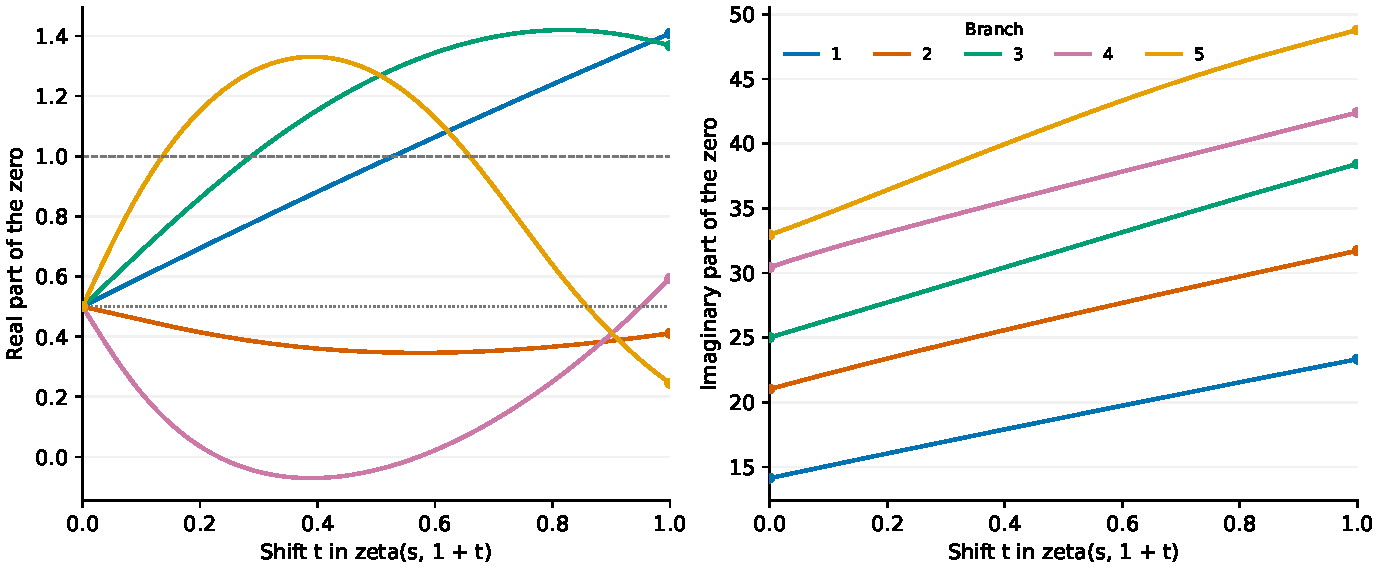
\includegraphics[width=\linewidth]{figures/hurwitz_paths.pdf}
\caption{The five certified branches as the first summand is removed. Curves join certified endpoint centres; the connecting segments are visual interpolation. The horizontal reference lines in the left panel are $\Re s=1/2$ and $\Re s=1$. Uniform disc certificates, rather than the drawn segments, prove continuation between the sampled points.}\label{fig:paths}
\end{figure}


\section{Effective signs and the inverse coefficient semiring}\label{sec:coefficient}
This section proves Theorem~\ref{thm:sign-main}. For a finite set $S\subset\Z$, put $F(S)=\Z^S$, using extension by zero for inclusions. The idempotent semiring is the finite-subset semiring $\B[\Z]$, with union and Minkowski sum. Convolution gives the maps
\[
 F(S)\otimes F(T)\longrightarrow F(S+T).
\]
They are associative and unital because integer convolution is. In Theorem 8.5 of \citet{CFMM}, this produces the elements $(S,c)$, with $c\in\Z^S$. Addition is union of the sets and extension-by-zero addition of coefficients; multiplication is Minkowski sum and convolution. A coefficient may be zero at a point of $S$. This is $\Z_0[q,q^{-1}]$.

\begin{proof}[Proof of the coefficient assertion in Theorem~\ref{thm:sign-main}]
For $a=a^++\eps a^-$ let $d=a^++a^-$ and $c=a^+-a^-$. Send $a$ to $(\supp d,c)$. Nonnegative coefficients give
\[
 \supp(d+d')=\supp d\cup\supp d',\qquad
 \supp(dd')=\supp d+\supp d'.
\]
The trace of a sum is $c+c'$, and the trace of a product is $cc'$ because $\eps^2=1$. These are exactly the operations just defined, including the empty support as zero.

Given $(S,c)$, choose at each $j\in S$ the multiplicities $(c_j,0)$ if $c_j>0$, $(0,-c_j)$ if $c_j<0$, and $(1,1)$ if $c_j=0$. Use $(0,0)$ outside $S$. This constructs a preimage and proves surjectivity.
\end{proof}

\begin{proposition}[Exact fibers]\label{prop:fibers}
Over a coefficient $c\ne0$ at an occupied weight, the possible dimensions are $|c|+2r$, $r\ge0$. Over an occupied coefficient $c=0$, they are $2r$, $r\ge1$. At an unoccupied weight the dimension must be zero. In particular the class $1+\eps$ maps to the old zero at weight $0$, while the empty class maps to $\tau$.
\end{proposition}
\begin{proof}
Solving $a^+-a^-=c$, $a^++a^-=d$ gives $a^\pm=(d\pm c)/2$. Nonnegativity, parity, and the requirement $d>0$ at occupied weights give exactly the listed alternatives.
\end{proof}

\begin{proof}[Proof of the descent assertions in Theorem~\ref{thm:sign-main}]
The classes $1+\eps$ and $2+2\eps$ have the same image, but have effective zeta functions $\zeta(s)L(s,\chi_{-4})$ and its square. Already the local factor at $5$ has exponent $2$ in the first and exponent $4$ in the second, so these formal Euler products differ. Their global functions differ as well: at $s=1$, $L(1,\chi_{-4})=\pi/4\ne0$, and the pole orders are one and two.

The trace $c$ is determined by $\pi(a)$, so any function or property of $c$ descends. This includes its trace zeta function, positivity in $\N[q+q^{-1}]$, and unimodality under any fixed convention for the Laurent coefficient sequence. In contrast take occupied weights $-2,-1,0,1,2$, with trace zero at each. The dimension sequences
\[
 (2,2,2,2,2)\quad\hbox{and}\quad(2,6,2,6,2)
\]
have the same image under $\pi$, but the first is unimodal and the second is not. Both come from effective classes by taking half the displayed dimension in each sign. Dimensions themselves therefore do not descend either.
\end{proof}

\begin{remark}[Cancellation pairs and supported zeros]
A cancelling pair added to a weight with a nonzero trace is lost under $\pi$, but does not create a supported zero at that weight. Thus the number of cancelling pairs and the number of occupied zero-trace weights are different invariants. An obstruction requiring extra cancelling pairs does not by itself prove that a coefficient of the inverse semiring is an old zero.
\end{remark}

\section{Witt multiplication and effective Euler factors}\label{sec:witt}
We use the standard big Witt ring $W(\Q)=1+T\Q[[T]]$. Its addition is multiplication of power series; its multiplication is characterized by
\[
 [a]\ast[b]=[ab],\qquad [a]=(1-aT)^{-1}.
\]
Its zero is the power series $1$ and its unit is $[1]$. This convention is the one used by \citet[\S1]{Ramachandran}.

\begin{proof}[Proof of Theorem~\ref{thm:witt-main}]
At an odd prime the assignments $q\mapsto[p]$ and $\eps\mapsto[\chi_{-4}(p)]$ preserve the relation $\eps^2=1$ and the inverse of $q$. The universal property of the group semiring gives a homomorphism. Its explicit formula is the one in the theorem. Taking the product over odd primes gives a homomorphism into the product of Witt rings.

At $p=3$, the rational numbers $3^j$ and $-3^j$, as $j$ ranges over $\Z$, are all distinct. Unique factorization of rational functions in $\Q(T)$ recovers the exponents $a_j^+$ and $a_j^-$ from $W_3(a)$. Hence the homomorphism is injective. Its image consequently determines $\pi(a)$, so $\pi$ factors through that image. The two classes in the previous proof show that the reverse factorization is impossible.

For unsigned Tate classes the same construction works at every prime, and the class $1$ gives $(1-T)^{-1}$ at each prime. Substituting $T=p^{-s}$ produces $\zeta(s)$. With $2$ excluded, the signed construction gives $\zeta^{(2)}(s)$ instead.

For the full signed Euler factors, the usual factor of $L(s,\chi_{-4})$ at $2$ is $1$, the Witt zero. Its Witt square is still $1$. But $\eps^2=1$ has factor $(1-T)^{-1}$ at $2$, the Witt unit. Thus preservation of multiplication fails at that prime. In representation-theoretic terms the quadratic sign character has zero inertia invariants at $2$, whereas its tensor square is trivial and has one-dimensional inertia invariants.
\end{proof}

For unsigned classes $c(q)=\sum a_jq^j$ with integral coefficients, the same formula extends to a ring map by allowing negative Witt sums. It is injective at any one fixed prime because the $p^j$ are distinct. Thus it is an isomorphism onto its image, not onto the whole Witt ring. A counted point adds $1$ to $c$, hence multiplies its global Euler product by $\zeta$. Tensoring by that point is the identity for Witt multiplication. These two operations explain the two uses of the word ``unit.''

The identity $\zeta_{\Q(i)}(s)=\zeta(s)L(s,\chi_{-4})$ can also be checked directly from prime splitting: at split primes it has two linear factors, at inert primes one quadratic factor, and at $2$ the ramified factor is $(1-2^{-s})^{-1}$. This is the zeta function of $\Spec\Z[i]$. The quotient image of its effective class is an occupied zero, but that single inverse-semiring element also represents every positive multiple of the class. It does not determine this particular scheme or its zeta function.

\section{Which arithmetic data ensure degree one?}\label{sec:degree}
The following statement separates an algebraic coefficient representation from its arithmetic realization.

\begin{proposition}\label{prop:degree}
Let a realization of $\mathcal E$ assign $q$ to the cyclotomic Tate character and $\eps$ to $\chi_{-4}$, with $q^j$ having geometric Frobenius eigenvalue $p^j$ at an unramified prime. Then every effective class has exactly the degree-one factors in Theorem~\ref{thm:sign-main}. More generally, a finite direct sum of rank-one characters of $G_{\Q}$ has a product of degree-one local factors. This conclusion uses the specified representations, not only the inverse-semiring pair $(\B[\Z],S\mapsto\Z^S)$.

Rationality of a coefficient over $\Q(D)$, $D=q+2+q^{-1}$, does not imply that it is the trace of a finite effective sign-Tate class.
\end{proposition}
\begin{proof}
Direct sums multiply characteristic polynomials, and a rank-one summand contributes a single factor $1-\chi(p)p^jT$. Substitution $T=p^{-s}$ proves the first assertion. Any tensor realization of the group semiring sends its group generators to tensor-invertible objects. A finite-dimensional tensor-invertible representation has dimension one, since the dimensions of it and its inverse multiply to one. This explains why a realization of this particular effective group semiring stays in rank one.

The inverse-semiring pair does not specify a Galois group, a representation, inertia, or Frobenius; these are additional data. For a concrete obstruction to the rationality assertion, $D^{-1}$ belongs to $\Q(D)$ but not to $\Z[q,q^{-1}]$. Indeed the only units of $\Z[q,q^{-1}]$ are $\pm q^m$, as follows by comparing lowest and highest exponents in a product equal to one. The polynomial $D$ is not such a unit. Every finite sign-Tate trace is an integral Laurent polynomial, so it cannot equal $D^{-1}$.
\end{proof}

Alp\"oge's theorem is taken here in precisely the Dirichlet form stated in his announcement \citep{Alpoge}: nontrivial zeros of Dirichlet $L$-functions lie on the critical line. It puts the nontrivial zeros of each explicitly occurring shifted factor on $\Re s=j+\tfrac12$. Finite-field weight purity is a different assertion: the eigenvalues $\pm p^j$ have absolute value $p^j$ directly, without a global Riemann hypothesis. The quotient $\pi$ remembers the set of weights, so it detects whether a nonempty object is concentrated in one weight. It does not remember its multiplicities.

For a different coefficient field or a non-Tate arithmetic realization, one must first specify the Galois representations. A Hecke character of a number field of degree $d$, viewed by induction over $\Q$, has degree $d$ before decomposition, even though it has rank one over the original field. A formal square root of $q$ supplies none of these data. Nor does a rational function of $D$ by itself supply a finite-dimensional representation. These are the exact additional gates in using a coefficient computation to select a Riemann hypothesis beyond the stated input.

\subsection{The pair attached to a specified representation category}
The coefficient field alone does not select a higher-degree replacement for the sign-Tate pair. A chosen semisimple representation category does give one explicitly.

Let $G$ be a finite group and $I$ its set of irreducible complex representations, with representatives $V_i$ and trivial representation $V_1$. Write
\[
 V_i\otimes V_j\cong\bigoplus_{k\in I} V_k^{\oplus N_{ij}^k},
 \qquad N_{ij}^k\in\N.
\]
Let $Q_G$ be the finite subsets of $I\times\Z$, with addition given by union, zero the empty set, and multiplication
\[
 S*T=\{(k,a+b): (i,a)\in S,\ (j,b)\in T,\ N_{ij}^k>0\}.
\]
Its unit is $\{(1,0)\}$. For $S\in Q_G$ put $F_G(S)=\Z^S$, with extension by zero along inclusions. The convolution of two coefficient vectors is
\[
 (c*d)_{k,n}=\sum_{a+b=n}\sum_{i,j\in I}N_{ij}^k c_{i,a}d_{j,b}.
\]
Only indices in their finite supports contribute.

\begin{proposition}[Fusion support and arithmetic degree]\label{prop:fusion-pair}
The operations above make $Q_G$ an idempotent semiring and $F_G$ an abelian-group-valued lax monoidal functor of the kind in \citet[Theorem 8.5]{CFMM}. Its inverse semiring consists of pairs $(S,c)$, $c\in\Z^S$, with the displayed convolution and support multiplication.

Let $\mathcal R_G^+$ be the semiring of finite direct sums of the symbols $V_iq^a$, using tensor decomposition for multiplication. The effective parity semiring
\[
 \mathcal E_G=\mathcal R_G^+[\eps]/(\eps^2-1)
\]
has a surjective homomorphism to this inverse semiring: at every index $(i,a)$ it records whether the sum of the two multiplicities is positive, and records their difference. An occupied coefficient may thus be zero.

For arithmetic realizations, choose an $\ell$-adic realization of the finite-group representations and an embedding of their algebraic character values into $\C$; the Tate character below is interpreted $\ell$-adically. Suppose in addition that a continuous surjection
$\operatorname{Gal}(\overline\Q/\Q)\twoheadrightarrow G$ is specified, $q$ is realized by the Tate character with unramified Frobenius eigenvalue $p$, and $\eps$ by a specified quadratic character. Then the irreducible effective constituents above an occupied $(i,a)$ have rank $\dim V_i$. At unramified primes their local factors have that degree. All such constituents have rank one if and only if every occupied $i$ is one-dimensional. This statement concerns the effective parity sectors, including occupied zero coefficients, rather than only their virtual signed difference.
\end{proposition}
\begin{proof}
Complete reducibility follows by averaging a projection over the finite group. Associativity and commutativity of tensor product give the corresponding equalities between sums of products of the nonnegative integers $N_{ij}^k$. Such a sum is positive exactly when at least one summand is positive. Taking supports of these identities proves associativity and commutativity of $*$, and distributivity over union. The trivial representation gives the claimed unit.

The convolution formula is bilinear and is compatible with extension by zero. Its associativity follows from the same tensor multiplicity identities, now as integer equalities; the coefficient of $V_1q^0$ supplies the unit constraint. These are precisely the lax monoidal identities. In the pair description, addition takes the union of supports and adds the extended vectors; multiplication is $(S,c)(T,d)=(S*T,c*d)$. The additive inverse is $(S,-c)$, so the additive monoid is inverse.

For multiplicities $p_{i,a},n_{i,a}\ge0$, put $u=p+n$ and $c=p-n$. Nonnegative convolution satisfies $\operatorname{supp}(u*v)=\operatorname{supp}(u)*\operatorname{supp}(v)$ because each $N_{ij}^k$ is nonnegative. The two sign evaluations give the usual sum and convolution identities for $u$ and $c$. Hence the stated map is a semiring homomorphism. To lift $(S,c)$, use $(p,n)=(c,0)$ where $c>0$, $(0,-c)$ where $c<0$, and $(1,1)$ at each occupied zero; outside $S$ use $(0,0)$. This proves surjectivity.

Inflation along a surjection preserves irreducibility: a subspace invariant under the Galois action is invariant under all of $G$. Tensoring with a character is an autoequivalence and preserves both irreducibility and dimension. Tate twists have the same property. An unramified local factor of $V_iq^a$ is
\[
 \det(1-p^a\rho_i(\operatorname{Frob}_p)T)^{-1};
\]
its denominator has degree $\dim V_i$ because Frobenius is invertible. A direct sum is a sum of rank-one constituents precisely when all its irreducible summands are one-dimensional. This gives the last assertion. At a ramified prime the degree is instead the dimension of the inertia-invariant subspace, so the unramified qualification is necessary.
\end{proof}

These are ordinary Artin local factors after the realization has been given; direct sums and their $L$-function factorizations are described by \citet[Remark 1.4, p.\ 203]{Sutherland}. Splitting a single local polynomial over $\C$ is not a decomposition into global rank-one representations. The latter must be compatible with every Galois element.

Two elementary examples show why rationality of coefficients cannot determine this degree. The quartic Dirichlet character modulo $5$ defined by $\chi(2)=i$ has values in $\Q(i)$ and rank one. In contrast the permutation representation of $S_3$ on $\Q^3$ has an invariant complement
\[
 V=\{(x_1,x_2,x_3):x_1+x_2+x_3=0\}
\]
of dimension two, with rational character $(2,0,-1)$ on the identity, transpositions, and three-cycles. It is irreducible over $\C$: a one-dimensional character is trivial on three-cycles, whereas the three-cycle on $V$ has the two primitive cube roots as eigenvalues. The splitting field of $X^3-2$ realizes this $S_3$ group, since the polynomial is Eisenstein at $2$ and its discriminant $-108$ is not a square. Thus rational characters already occur at rank two. Tensoring this representation with the quartic character gives a rank-two example with the same nonrational character field $\Q(i)$ as the rank-one example. Indeed, the splitting field of $X^3-2$ has unique quadratic subfield $\Q(\sqrt{-3})$, whereas the cyclic quartic field $\Q(\zeta_5)$ has quadratic subfield $\Q(\sqrt5)$. Their intersection is therefore $\Q$: a common quotient of $S_3$ and $C_4$ would otherwise be quadratic. The compositum has group $S_3\times C_4$, and an element trivial on the first factor with $\chi=i$ has trace $2i$. Thus the character field is exactly $\Q(i)$.

For the finite-image representations just used, unramified Frobenius eigenvalues are roots of unity, so the Tate-twisted local eigenvalues have absolute value $p^a$. This local purity follows directly from finite order. A statement that all nontrivial global zeros lie on the corresponding critical line is a separate Artin or Hecke Riemann hypothesis. The specified Dirichlet input addresses rank-one characters over $\Q$; it does not by itself establish that higher-rank assertion. For more general arithmetic categories one must provide their representations, tensor rules, and weight theorem first. An algebraic coefficient over $\Q(D)$ supplies none of those choices uniquely.


\section{Divisor supports as Boolean sheaves}\label{sec:sheaves}
This section isolates what depends on the zero-adjoined construction in divisor and packet descriptions. Let $X=\C$, let $Z\subset X$ be closed and discrete, and let $m_z\ge1$ be integers. Regard $\B=\{\tau,e\}\subset\C_0$ as a semiring with unit $e$; its inclusion is not a unital map to $\C_0$. Its semimodules are join-semilattices with zero.

\begin{theorem}\label{thm:divisor}
The presheaf
\[
 U\longmapsto\bigoplus_{z\in U\cap Z}\B^{m_z}
\]
of finite-support sections sheafifies to $\mathcal V(U)=\prod_{z\in U\cap Z}\B^{m_z}$. Its stalk is $\B^{m_z}$ at $z$ and a singleton off $Z$. The reduced sheaf $\mathcal A(U)=\prod_{z\in U\cap Z}\B$ is a canonical retract of $\mathcal V$, by the join and diagonal maps. It is isomorphic to $\mathcal V$ precisely when every $m_z=1$.

For the truncated discrete valuation ring $\C[t]/(t^m)$, the ideal lattice is a chain of $m+1$ elements, whereas $\B^m$ is a Boolean lattice of $2^m$ elements. The chain embeds as the tails of $\{1,\ldots,m\}$ and has both a left and a right order adjoint. Thus these two encodings recover $m$ but are different when $m>1$.
\end{theorem}
\begin{proof}
A product of sections over points glues uniquely coordinate by coordinate, so $\mathcal V$ is a sheaf. Every point of $Z$ has a neighborhood meeting $Z$ in that point alone, and every point off $Z$ has a neighborhood avoiding $Z$. The finite-support presheaf and the product sheaf have the same stalks on those neighborhoods; the indicated map therefore induces an isomorphism on sheafification.

Identify $\B^m$ with subsets of $\{1,\ldots,m\}$, using union as addition. The join map sends a nonempty subset to $1$ and the diagonal sends $1$ to the full set. Their composite is the identity on $\B$. Applying this coordinatewise gives the retract. If the sheaves are isomorphic, their stalk cardinalities give $2^{m_z}=2$, hence $m_z=1$; the converse is immediate.

Every nonzero ideal of $\C[t]/(t^m)$ has an element of least $t$-adic order $k<m$. Its unit multiple generates $(t^k)$; every element of the ideal has order at least $k$, proving the classification, including the zero ideal $(t^m)$. The chain of tails contains both endpoints. The least tail containing a subset is its left order adjoint, and the largest tail contained in a subset is its right order adjoint: these are exactly the defining containment equivalences. Cardinality proves the last distinction.
\end{proof}

\begin{proposition}[The compactification stalk]\label{prop:tail}
Let $j:\C\hookrightarrow\mathbf P^1(\C)$, and attach pointed sets $M_z$ to a closed discrete set $Z$. For the product sheaf $\mathcal F(U)=\prod_{z\in U\cap Z}M_z$, the stalk of $j_*\mathcal F$ at infinity consists of sequences modulo agreement outside a finite set. The stalk of $j_!\mathcal F$ there is the one-point set. For abelian groups this is the quotient $\prod M_z/\bigoplus M_z$.
\end{proposition}
\begin{proof}
A compact subset of $\C$ meets a closed discrete set in finitely many points. Conversely any finite subset of $Z$ lies in a compact disc. Neighborhoods of infinity consequently form, on $Z$, the cofinite filter. Taking the direct limit of the products over these neighborhoods identifies two sections exactly when they agree off a finite set. Extension by zero has zero stalk at every point of the complement by its definition. In groups, the equivalence relation has kernel precisely the finitely supported subgroup.
\end{proof}

If a finite group permutes $Z$ and preserves $m_z$, the invariants in the pushforward to the orbit set have one stalk $\B^{m_z}$ for each orbit: an invariant tuple is constant along the orbit. This is ordinary descent for a permutation action with trivial stabilizer action on the displayed fiber. A nontrivial stabilizer action must instead be included in the invariants. Applying these constructions to the zero divisor of a meromorphic function is legitimate, but supplies no new theorem on the location, simplicity, or multiplicity of its zeros. Product expansions and logarithmic derivatives of $\zeta$ that do not use $R_0$ belong to analytic number theory separately.

\subsection{Jet coefficients and Boolean support}

The ideal-chain comparison has a second, coordinate-dependent companion. Fix a centered coordinate $t=s-x$ at a point of multiplicity $m\geq1$, and put
\[
 E_m=t\C[t]/(t^{m+1}),\qquad J_m=\C[t]/(t^m).
\]
The first is a pointed vector space, with ordered basis $t,\ldots,t^m$. Identify $\B^m$ with the subsets of $\{1,\ldots,m\}$ as in Theorem~\ref{thm:divisor}.

\begin{proposition}[The precise jet-support map]\label{prop:packet-jet-support}
The maps
\[
 \kappa_m\!\left(\sum_{r=1}^m c_rt^r\right)
       =\{r:c_r\ne0\},\qquad
 \iota_m(I)=\sum_{r\in I}t^r
\]
are maps of pointed sets and satisfy $\kappa_m\iota_m=\operatorname{id}$. The fibre of $\kappa_m$ over $I$ is $(\C^\times)^I$, with a singleton fibre over the empty set. The map $\kappa_m$ is not additive, and the additive monoids of $E_m$ and $\B^m$ are not isomorphic.

Division by the chosen coordinate gives a linear isomorphism $d_m:E_m\to J_m$. It takes $\C t^m$ onto the socle $\{a\in J_m:ta=0\}=\C t^{m-1}$. If a holomorphic germ $f$ has order $m$ at $x$, then
\[
 [f]=\frac{f^{(m)}(x)}{m!}t^m\ne0
       \quad\text{in }E_m.
\]
Its Boolean support is $\{m\}$, and $d_m[f]$ generates the socle of $J_m$.
\end{proposition}
\begin{proof}
The displayed basis gives unique coefficients, so support and the section are well defined. Prescribing the nonzero coefficients exactly at the indices in $I$ gives the stated fibre. However, $t$ and $-t$ both have support $\{1\}$, whereas their sum has empty support. Thus support fails to preserve addition. Every element of the target is additively idempotent, while $t+t\ne t$ in $E_m$, ruling out an additive-monoid isomorphism.

The map $d_m$ lowers every exponent by one and has inverse multiplication by $t$ followed by reduction modulo $t^{m+1}$. In $J_m$, multiplication by $t$ kills precisely the coefficient line of $t^{m-1}$. Finally the definition of vanishing order and Taylor expansion give
$f(s)=f^{(m)}(x)t^m/m!+O(t^{m+1})$, with nonzero leading coefficient. This proves all remaining assertions.
\end{proof}

For a closed discrete divisor, these maps assemble coordinatewise into maps of product sheaves. The support retraction is a retraction of pointed sheaves. It does not identify the vector-space jet sheaf with a Boolean semimodule sheaf. The order of vanishing and the socle line are intrinsic; the support of a general coefficient vector depends on the chosen coordinate. Divisor addition also has a direct Boolean interpretation: concatenation gives $\mathcal V_{D_1+D_2}\cong\mathcal V_{D_1}\times\mathcal V_{D_2}$. For disjoint supports this is simply the separation of the corresponding factors.

The Boolean coordinates also have their ordinary polynomial meaning. For every commutative $\B$-algebra $A$, evaluation gives
\[
 \operatorname{Hom}_{\B\text{-alg}}(\B[T_1,\ldots,T_m],A)
       \cong A^m.
\]
An image of each variable determines exactly one homomorphism, by the polynomial universal property. On $\B$-valued points, the substitutions $T_j\mapsto T$ and $T\mapsto T_1+\cdots+T_m$ induce the diagonal and join maps. Their composite sends $T$ to $mT=T$ in the idempotent polynomial semiring, so the retraction is already realized by these polynomial maps. This does not make the join map $\B^m\to\B$ a semiring homomorphism: for $m\geq2$, two disjoint nonempty coordinate supports have zero coordinatewise product but their joins both equal $1$.

An endpoint-label construction is equally explicit. In the two-dimensional space of principal parts
\[
 V=\C\frac{ds}{s}\oplus\C\frac{ds}{s-1},
\]
the residues at $0,1$ identify $V$ with $\C^2$. Subsets of $\{0,1\}$ correspond exactly to its coordinate subspaces. Thus the support map from $R_0^2$ to these four subspaces forgets precisely the coefficient fibre $R^I$ above the support $I$. If
\[
 q(s)=\frac1{s(s-1)},\qquad
 \ell(s)=\frac1s+\frac1{s-1},
\]
then $Aq(s)ds+B\ell(s)ds$ has residues $(-A+B,A+B)$; the inverse is $A=(b-a)/2$, $B=(a+b)/2$. Pullback by $s\mapsto1-s$ exchanges the endpoint basis forms. These are linear and support-coordinate identities, with no additional analytic information about a divisor.

\subsection{Descent and phase decorations}

The stabilizer qualification in the permutation construction can be stated explicitly.

\begin{proposition}[Invariant pushforward on a discrete orbit space]\label{prop:packet-stabilizer}
Let a finite group $G$ act on a discrete set $Z$, and suppose pointed sets or algebraic objects $M_z$ have compatible transport isomorphisms $M_z\to M_{gz}$. Let $q:Z\to Z/G$. For the product sheaf $\mathcal F$ and an orbit $O=Gz$,
\[
 (q_*\mathcal F)^G_O\cong M_z^{G_z},
 \qquad G_z=\{g:gz=z\}.
\]
For permutation-only transport on $\B^{m_z}$, with multiplicity constant on each orbit, this is the diagonal copy of $\B^{m_z}$. The same statement holds for the chain of ideals of $J_{m_z}$, and its two adjoints to the Boolean-cube inclusion descend coordinatewise.
\end{proposition}
\begin{proof}
The quotient of a discrete space is discrete, so the stalk over $O$ is the product of its fibres. A $G$-invariant tuple is determined by its $z$-coordinate, and invariance forces that coordinate to be fixed by $G_z$. Conversely, given $a\in M_z^{G_z}$, assign $ga$ to the coordinate $gz$. If $gz=hz$, then $h^{-1}g\in G_z$, so the assignment is independent of the representative. The two constructions are inverse and preserve every given operation. With permutation-only transport the stabilizers act trivially. The chain-cube maps depend only on $m_z$, so they commute with transport and restrict to invariants.
\end{proof}

This construction applies to any multiplicity-preserving symmetry of a divisor. For completed-zeta packets it uses the ordinary conjugation and functional-equation symmetries; it provides no additional assertion about zero locations.

There is also a precise pointed-set meaning for a phase decoration. Set $M=\{*\}\sqcup S^1$, pointed at $*$, and define
\[
 \pi(*)=0,\quad \pi(z)=1\ (z\in S^1),\qquad
 \iota(0)=*,\quad \iota(1)=1\in S^1.
\]
Then $\pi\iota=\operatorname{id}_{\B}$. On a closed discrete set, products give a split map of pointed sheaves from $\prod M$ to $\prod\B$, with fibre $S^1$ over an occupied Boolean coordinate. At the simple zeros of a fixed-coordinate holomorphic function, the values $f'(x)/|f'(x)|$ give a section. This assertion supplies a pointed decoration; it does not equip $M$ with an inverse-semiring module structure. In particular, analytic phase-product identities require their own analytic hypotheses and do not follow from the Boolean support map.

\subsection{The vector tail has no additional higher cohomology}

For completeness, the vector-space counterpart of Proposition~\ref{prop:tail} identifies the cohomology of the finite-support extension.

\begin{proposition}[Tail exact sequence]\label{prop:packet-tail-exact}
Let $Z\subset\C$ be closed and discrete, let $V_z$ be complex vector spaces, and let $\mathcal F(U)=\prod_{z\in U\cap Z}V_z$. Put
\[
 T=\left(\prod_{z\in Z}V_z\right)
       \Big/\left(\bigoplus_{z\in Z}V_z\right).
\]
For $j:\C\hookrightarrow\mathbf P^1(\C)$ and $i_\infty:\{\infty\}\hookrightarrow\mathbf P^1(\C)$ there is an exact sequence
\[
 0\longrightarrow j_!\mathcal F\longrightarrow j_*\mathcal F
   \longrightarrow i_{\infty*}T\longrightarrow0.
\]
Moreover $H^q(\mathbf P^1(\C),j_!\mathcal F)=0$ for every $q\geq1$.
\end{proposition}
\begin{proof}
On an open set containing infinity, the extension by zero consists of the finite-support families. Indeed its support must avoid some neighborhood of infinity, and a compact set meets $Z$ in finitely many points. On an open set avoiding infinity it is the unrestricted product sheaf. These rules give a sheaf: in a cover of a neighborhood of infinity, choose one member containing infinity; only finitely many support points lie outside that member, so gluing preserves finite support.

The map to the tail class on neighborhoods of infinity, and the zero map on other opens, is compatible with restriction. Its stalk kernel is $j_!\mathcal F$ by Proposition~\ref{prop:tail}; its stalk map at infinity is surjective, and all other target stalks vanish. This proves exactness. Both $j_*\mathcal F$ and $i_{\infty*}T$ are flasque, since their restriction maps are coordinate projections or identity and zero maps. Flasque sheaves are acyclic \citep[Lemma 20.12.3, Tag 09SY]{StacksFlasque}. Their long exact cohomology sequence gives the required vanishing in degrees at least two. In degree one it remains to observe that the global map $\prod V_z\to T$ is surjective by the definition of $T$. This proves the degree-one assertion as well.
\end{proof}


\section{The monoid zeta obstruction}\label{sec:deitmar}
Deitmar's definition starts with finite-type monoid schemes and a zeta polynomial obtained from finite-field point counts subject to a torsion condition \citep[Theorem 1 and \S\S1--2]{Deitmar}. It is not the product obtained by assigning each prime monoid ideal the order of its unit group.

\begin{proposition}[Prime ideals of the pointed multiplicative monoid]\label{prop:monoid-spectrum}
Let $M_0$ be the pointed multiplicative monoid underlying $\Z_0$, with new absorbing element $\tau$. Its prime monoid ideals are $\{\tau\}$ and
\[
 P_A=\{\tau,0_\Z\}\cup
 \{n\in\Z\setminus\{0\}:\text{some prime in }A\text{ divides }n\},
\]
one for each subset $A$ of the rational primes, including the empty subset. In particular its monoid spectrum has infinite Krull dimension, and $M_0$ is not Noetherian.
\end{proposition}
\begin{proof}
A monoid ideal contains $\tau$ and is closed under multiplication by arbitrary elements. Its complement must be multiplicatively closed for it to be prime. The set $\{\tau\}$ is prime because products of old ring elements remain old ring elements.

Any larger ideal contains an old integer and hence contains $0_\Z$. A proper ideal contains neither $1$ nor $-1$. By unique factorization of a nonzero integer, primeness then says that it belongs to the ideal exactly when one of its prime divisors does. Thus the ideal is $P_A$, where $A$ is its set of positive prime elements. Conversely the displayed $P_A$ is an ideal and its complement is multiplicatively closed, so it is prime.

Enumerating the rational primes produces arbitrarily long strict chains of the $P_A$, proving infinite dimension. The monoid ideal generated by the first $n$ primes consists of $\tau$, the old zero, and their integer multiples. The next prime belongs to the next such ideal and not the preceding one. These ideals form a strictly ascending infinite chain, proving the failure of the ascending-chain condition.
\end{proof}

The additive semiring spectrum of $\Z_0$ and this multiplicative monoid spectrum are different constructions. Forgetting addition creates all the extra prime ideals $P_A$; it does not preserve the finite-dimensional prime-chain structure of the additive semiring spectrum.


\begin{proposition}\label{prop:deitmar}
Let $M$ be the multiplicative monoid of $\Z$, considered in Deitmar's unpointed-monoid convention, or equivalently contract only the newly adjoined $\tau$ in the multiplicative monoid of $\Z_0$. Its base-change algebra is
\[
 \Z[M]\cong\Z\times\Z[C_2][x_p:p\text{ prime}].
\]
It is not of finite type and has infinitely many points over every finite field. Thus Deitmar's finite-type zeta-polynomial construction does not assign to this object the function $(1-2^{-s})^{-1}$.

If only $r$ prime generators are allowed, the finite approximation has $1+\gcd(2,q-1)q^r$ points over $\mathbf F_q$. Its Deitmar zeta polynomial is $1+q^r$, using exponent $2$ in the torsion condition.
\end{proposition}
\begin{proof}
Write $z$ for the basis element of the monoid algebra corresponding to the integer zero. It is a central idempotent and satisfies $z[m]=z$ for every $m$. The factor $z\Z[M]$ is a copy of $\Z$. In the complementary factor, the nonzero integers form the free commutative monoid on the positive primes times the group $\{\pm1\}$. This gives the displayed product decomposition. The polynomial algebra on infinitely many independent variables is not finitely generated. Assigning each $x_p$ independently a value in a finite field already gives infinitely many points.

For $r$ variables the first factor contributes one point. The second contributes one choice of a root of $u^2=1$ and arbitrary choices for the $r$ variables. The number of such roots is $\gcd(2,q-1)$. When $\gcd(2,q-1)=1$, the count is $1+q^r$, as asserted.
\end{proof}

In the sign convention printed in \citet[p.\ 1]{Deitmar}, the finite approximation therefore has $\mathbf F_1$-zeta $s(s-r)$; with the reciprocal convention used in much later literature it has $1/[s(s-r)]$. Neither convention yields the previously proposed Euler factor. Keeping track of the convention and of finite type is essential here.

\section{Questions left by these results}
The quotient identities and coefficient descent statements are exact. The five branches in Theorem~\ref{thm:paths-main} have certified simplicity and continuation, but the corresponding assertion for every Hurwitz-zero branch remains open here. Multiple zeros and escape to infinity are the possible obstructions outside the certified branches. The asymptotic proportion of simple zeros initially moving right also remains open: Proposition~\ref{prop:zero-phase} reduces it to a modulo-two phase-distribution condition which a normalized central limit theorem does not establish.

A proposed first-moment asymptotic for the initial velocities also remains unproved. Summing the simple-zero formula over every zero first requires simplicity, or a definition and analysis of the aggregate motion at multiple zeros. A zero-location hypothesis alone does not supply that condition or the necessary reciprocal-derivative and contour estimates.

For applications to canonical bases, an associative algebra with Laurent coefficients must still be lifted to effective classes. Denominators in a rational coefficient field must first be removed or supplied with a separate arithmetic interpretation. An inverse-semiring description alone determines neither that lift nor the Galois representations needed for a higher-degree $L$-function. Likewise, a Boolean sheaf attached to a known divisor records that divisor but does not construct its zeros.

Proposed support lifts of analytic packets, conormal quotients and primitive corrections require further data. One must specify source and target join-semilattices, compatible group diagrams and scalar actions, a join-preserving support map, and linear fiber maps commuting with transitions and scalar action. A scalar coefficient identity or a Hilbert-space norm decomposition does not specify these data. Constructing the arithmetic diagrams and the compatible maps remains a separate open problem.

\section*{Note on method}
The zero-adjoined construction and the inverse-additive-monoid theorem are due to \citet[Definition 3.6 and Proposition 6.1]{FGJM}, whose 2024 paper precedes the project's independent development. The latter began in a conversation with Gemini 2.5 Pro in the Gemini app and was formalized by Gemini 2.5 Deep Think in that app's Deep Think mode in November 2025; versions were deposited as HI-AI on Zenodo from 6 November 2025 and later withdrawn. The project continued with a GPT-5-series Pro extraction in ChatGPT Pro mode at reasoning effort ultra in March 2026, a corpus by those models at ultra from April to July, and Codex work at ultra in August and September. Notes of 21--23 November were by Claude Opus 5.5 at max, with consults by Claude Fable 5.2 at max and Claude Opus 5.5 at high. Those earlier materials are unpublished project notes, not independent literature. This text and its mathematical checks were produced by GPT-6 Astra Pro; the numerical effort setting is not exposed. Separate re-proofs use the same model and are not human review. No human has checked this text. The newly written text and programs are dedicated to the public domain under CC0 1.0. The subject workbench is \url{\workbenchurl}, and the permanent record address is \url{\recordurl}.

\begin{thebibliography}{99}
\bibitem[\emph{Spectrum, semimodules and projectives}(2026)]{FoundationPublic}
\emph{Spectrum, semimodules and projectives of the inverse semiring $R_0$ of Faul, Goswami, Joubert and Manuell}. (2026, November 24).
Hexagon, 2611.00993v1. \url{https://hexagonmath.org/2611.00993v1}.
\bibitem[Alp\"oge(2026)]{Alpoge} Alp\"oge, L. (2026, November 20). \emph{Remark on the Riemann hypothesis}. \url{https://alpo.ge/remark.pdf}. Announcement and linked Lean archive; Dirichlet Riemann hypothesis used as external input.
\bibitem[Caviglia et al.(2026)]{CFMM} Caviglia, E., Faul, P. F., Manuell, G., \& Mesiti, L. (2026). \emph{Clifford semigroups and the monoidal Grothendieck construction} (Version 2). arXiv:2607.12944. \url{https://arxiv.org/abs/2607.12944}.
\bibitem[Davenport and Heilbronn(1936a)]{DH1} Davenport, H., \& Heilbronn, H. (1936a). On the zeros of certain Dirichlet series. \emph{Journal of the London Mathematical Society, s1-11}(3), 181--185. \url{https://doi.org/10.1112/jlms/s1-11.3.181}.
\bibitem[Davenport and Heilbronn(1936b)]{DH2} Davenport, H., \& Heilbronn, H. (1936b). On the zeros of certain Dirichlet series, II. \emph{Journal of the London Mathematical Society, s1-11}(4), 307--312. \url{https://doi.org/10.1112/jlms/s1-11.4.307}.
\bibitem[Deitmar(2006)]{Deitmar} Deitmar, A. (2006). \emph{Remarks on zeta functions and K-theory over $\mathbf F_1$}. arXiv:math/0605429v3. \url{https://arxiv.org/abs/math/0605429}.
\bibitem[Faul et al.(2024)]{FGJM} Faul, P. F., Goswami, A., Joubert, G., \& Manuell, G. (2024). \emph{The case for inverse semirings}. arXiv:2411.12318. \url{https://arxiv.org/abs/2411.12318}.
\bibitem[Johansson(2015)]{Johansson} Johansson, F. (2015). Rigorous high-precision computation of the Hurwitz zeta function and its derivatives. \emph{Numerical Algorithms, 69}, 253--270. \url{https://doi.org/10.1007/s11075-014-9893-1}. Preprint arXiv:1309.2877.
\bibitem[Levinson(1975)]{Levinson} Levinson, N. (1975). Almost all roots of $\zeta(s)=a$ are arbitrarily close to $\sigma=1/2$. \emph{Proceedings of the National Academy of Sciences, 72}(4), 1322--1324. \url{https://doi.org/10.1073/pnas.72.4.1322}.
\bibitem[Ramachandran(2015)]{Ramachandran} Ramachandran, N. (2015). Zeta functions, Grothendieck groups, and the Witt ring. \emph{Bulletin des Sciences Math\'ematiques, 139}(6), 599--627. \url{https://arxiv.org/abs/1407.1813}.
\bibitem[The Stacks Project Authors(2026)]{StacksFlasque}
The Stacks Project Authors. (2026). \emph{The Stacks Project}, Lemma 20.12.3, Tag 09SY (Flasque sheaves are acyclic). \url{https://stacks.math.columbia.edu/tag/09SY}.
\bibitem[Neukirch(1999)]{NeukirchShift}
Neukirch, J. (1999). \emph{Algebraic number theory} (N. Schappacher, Trans.).
Springer. \url{https://doi.org/10.1007/978-3-662-03983-0}.
Chapter VII, \S5, Proposition 5.2 and Corollary 5.11.

\bibitem[Sutherland(2019)]{Sutherland}
Sutherland, A. V. (2019). Sato--Tate distributions. \emph{Contemporary Mathematics, 740}, 197--248. \url{https://doi.org/10.1090/conm/740/14904}.

\bibitem[National Institute of Standards and Technology(2026a)]{DLMFShift}
National Institute of Standards and Technology. (2026a).
\emph{Digital Library of Mathematical Functions}, \S25.11(i),
equations 25.11.1, 25.11.14, 25.11.17, and 25.11.18.
\url{https://dlmf.nist.gov/25.11}. Retrieved November 24, 2026.

\bibitem[National Institute of Standards and Technology(2026b)]{DLMFZeros}
National Institute of Standards and Technology. (2026b). \emph{Digital Library of Mathematical Functions}, \S25.10(i), equations 25.10.1--2. \url{https://dlmf.nist.gov/25.10}.
\bibitem[Arias de Reyna and van de Lune(2011)]{AriasLune}
Arias de Reyna, J., \& van de Lune, J. (2011). \emph{Some bounds and limits in the theory of Riemann's zeta function}. arXiv:1107.5134v1. Theorems 3.1 and 4.1, pp.~4--5. \url{https://arxiv.org/abs/1107.5134}.
\bibitem[National Institute of Standards and Technology(2026c)]{DLMFReflection}
National Institute of Standards and Technology. (2026c).
\emph{Digital Library of Mathematical Functions}, equations 25.4.3--25.4.4.
\url{https://dlmf.nist.gov/25.4}. Retrieved November 24, 2026.

\end{thebibliography}
\end{document}
